\section{Statistics and Parameters}

In this section, we discuss the process of going from sky maps at different frequencies---or, in light
of the previous section, foreground-cleaned CMB maps and an estimate of foreground residuals---to
post-map products such as angular power spectra, estimates of lensing potential $\phi$, and finally
cosmological parameters, as well as covariance estimates for all of these quantities. We briefly describe
the current practice for this process, then we address specific challenges anticipated in the \cmbexp\ era.
%
%
%? Current practice for going from frequency maps, or cleaned CMB maps, plus noise description, to lensing power spectra and (lensed) TT, TE, EE, BB power spectra, and parameters
%
%	? CMB power spectra
%		How is map noise treated?
%		How is foreground-related uncertainty treated?
%			? galactic  (include BKP description of BKP work)
%			? extragalactic
%
%	? Lensing power spectra
%
%? Challenges to reducing CMB-S4 data to cosmological parameter estimates
%
%	? Foreground-cleaning will be very important for r
%	? Delensing will be important for studying the tensor signal, or setting tightest possible upper limit
%	? Quadratic estimator will be highly suboptimal at S4 noise levels
%	? Lensed power spectra and reconstructed lensing power will have lensing potential sample variance as source of correlated uncertainty
%
%? Paths toward meeting these challenges
%

\begin{figure}[htbp]
\centering
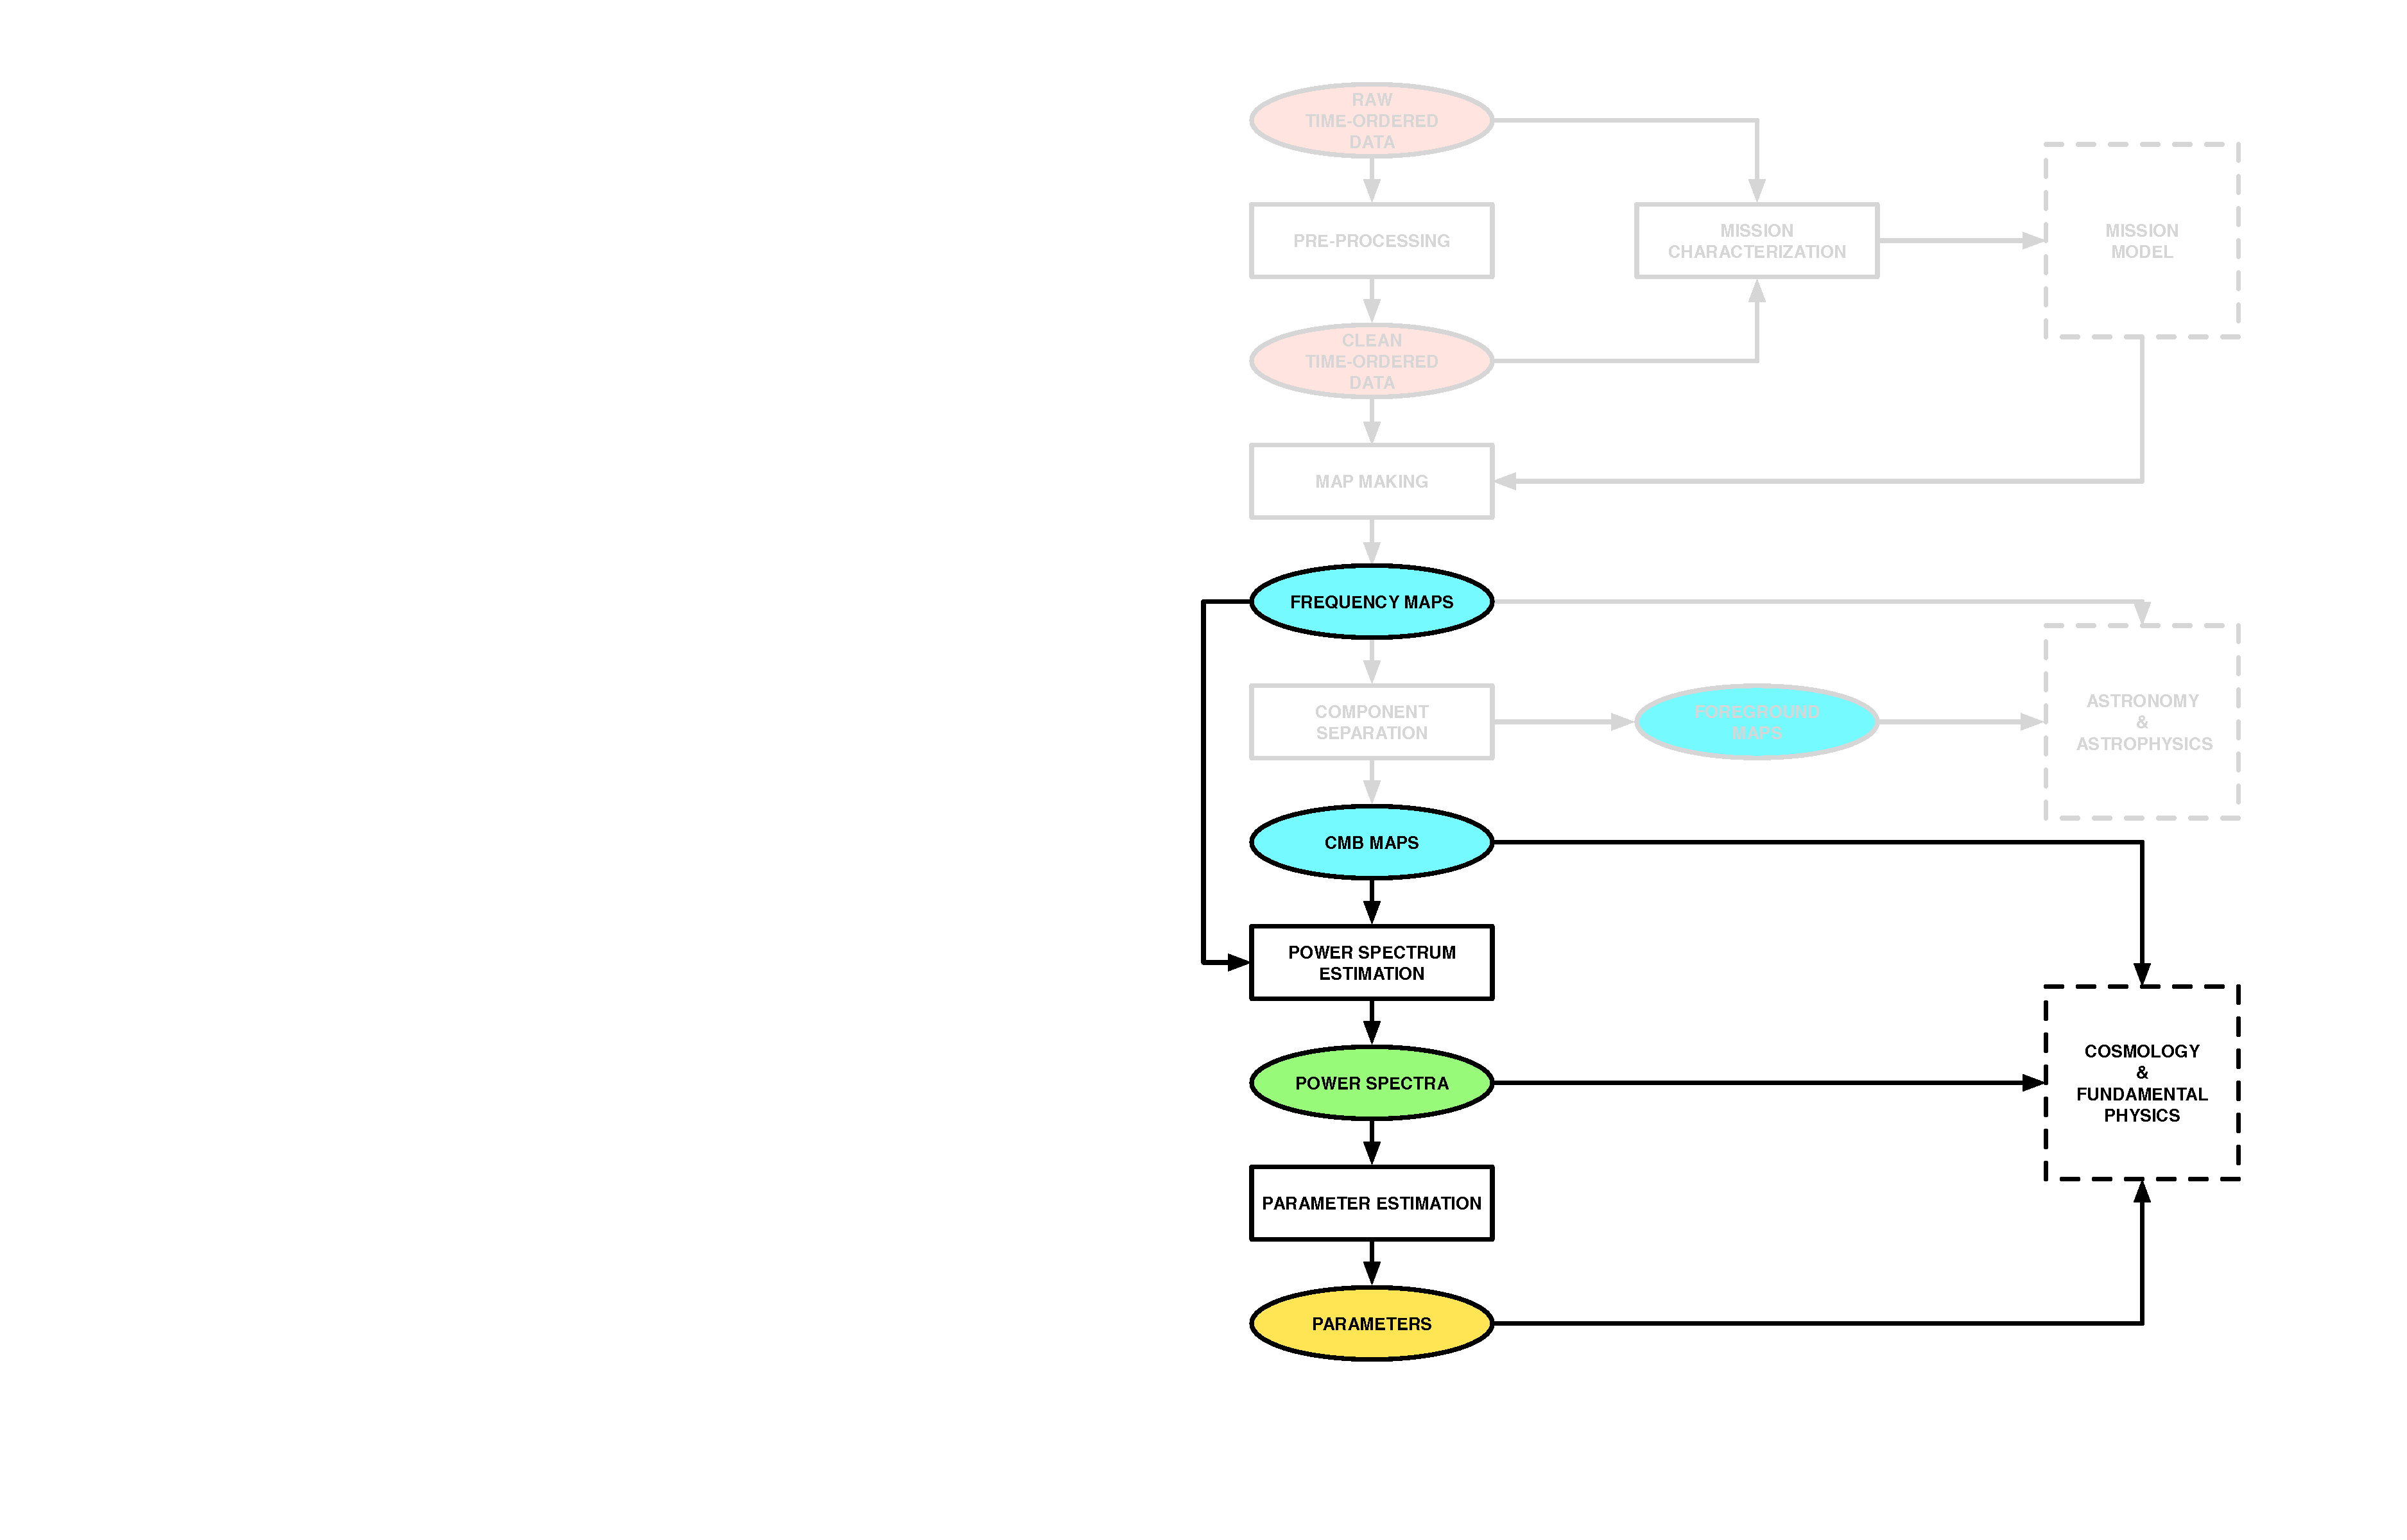
\includegraphics[width=0.5\textwidth]{Analysis/sp}
\caption{The statistics and parameters subset of the CMB data analysis pipeline}
\label{fig_sp}
\end{figure}


\subsection{Current practice}
\label{se:current}
Early measurements of CMB temperature anisotropy, with comparatively few map pixels or angular modes
measured, often used maximum-likelihood methods to produce maps of the sky (e.g., \cite{wright96}) and
either a direct evaluation of the full likelihood or a quadratic approximation to that likelihood (e.g., \cite{bond98a}) to go from 
maps to angular power spectra (the first step in Figure \ref{fig_sp}). With the advent of the WMAP and Planck space 
missions, which would map the entire sky at sub-degree resolution, it became apparent that computing
resources could not compete with the $\mathcal{O}({\cal N}^3)$ scaling of the full-likelihood approach 
(e.g., \cite{borrill99}). The solution for power spectrum analysis
that has been adopted by most current CMB experiments is a
Monte-Carlo-based approach advocated in \cite{hivon02}. In this approach, a biased estimate of
the angular power spectrum of the data is obtained by simply binning and averaging the square 
of the spherical harmonic transform of the sky map. That estimate (known as the 
``pseudo-$C_\ell$ spectrum'') is related to the unbiased 
estimate that would be obtained in a maximum-likelihood procedure through the combined effect
of noise bias, sky windowing, and any filtering applied to the data before or after mapmaking
(including the effects of instrument beam and pixelization). These effects are estimated by ``observing''
and analyzing simulated data and constructing a matrix describing their net influence on simulated data. 
This matrix is inverted, and the inverse matrix is applied to the pseudo-$C_\ell$s to produce the 
final data product. Some version of this Monte-Carlo treatment is likely to be 
adopted for \cmbexp. 

Pseudo-$C_\ell$ methods are also now commonly used in analysis of CMB polarization anisotropy
\cite{planck15-11,naess14,crites15}. An added complication in polarization analyses is that 
pseudo-$C_\ell$ methods do not cleanly separate $E$ and $B$ modes (e.g., \cite{challinor05}).
``Pure'' $B$-mode estimators can be constructed that suppress the spurious $B$-mode contribution
from estimating $E$ and $B$ on a cut sky with pseudo-$C_\ell$ methods \cite{smith06}), but 
other analysis steps (such as particular choices of filtering) can produce spurious $B$ modes that
are immune to the pure estimators \cite{keisler15}. These can also be dealt with using Monte-Carlo
methods, either by estimating the statistical bias to the final $B$-mode spectrum or by constructing
a matrix representing the effect of any analysis steps on the true sky \cite{BICEP2014}. The latter
approach involves constructing an ${\cal N}_\mathrm{pixel}$-by-${\cal N}_\mathrm{pixel}$ matrix, equal in size to the 
full pixel-pixel covariance, and will not be feasible for high-resolution \cmbexp\ data but could be 
used in analyzing lower-resolution data.

In addition to the two-point function of CMB maps, higher-order statistics of the maps have recently 
been of great interest to the community. In particular, the four-point function encodes the effect of 
gravitational lensing, and estimators can be constructed to go from CMB temperature and polarization
maps to estimates of CMB lensing $\phi$ and the associated covariance (e.g., \cite{hu02a,okamoto03}).
These quadratic estimators are the first step in an iterative estimation of the true likelihood, and in
the weak-lensing limit they are nearly optimal; as a result, they remain the state of the art for estimating
the large-scale $\phi$ from CMB lensing (e.g., \cite{planck13-18}). For \cmbexp\ sensitivity levels, 
it is possible that further gains can be made with more iterations (see Section \ref{delens}).
Even with multiple steps, the computational burden involved
in this step of the analysis is unlikely to be significantly greater for \cmbexp\ than for Planck.

The final step in the analysis of a CMB data set is the estimation of cosmological parameters from
the various post-map statistics discussed above (the second step in Figure \ref{fig_sp}). This involves estimating the likelihood of the data
given a model parameterized by the standard six $\Lambda$CDM parameters, possible extensions
of the cosmological model, and any nuisance parameters involving the instrument, foregrounds, and
other sources of systematic uncertainty. The current industry standard for this part of the analysis are
Monte-Carlo Markov-Chain (MCMC) methods, in particular the implementation in CosmoMC
\cite{lewis02b}, and it is expected that \cmbexp\ will use similar methods. There will be several 
aspects of the \cmbexp\ dataset, however, that will necessitate going beyond what past analyses
have done at this step. First of all, the data from several different telescopes and cameras will need
to be combined in as lossless a fashion as possible---such that combining at the parameters stage
may be sub-optimal.
Further, as shown by \cite{bicepkeckplanck15}, foregrounds cannot be ignored in the 
estimation of the $B$-mode power spectrum, even in the cleanest parts of the sky and in the 
least contaminated observing bands. Foreground modeling will be used to mitigate the contamination,
but there will be foreground residuals (both from noise and imperfect modeling), and these need
to be properly characterized and accounted for in parameter extraction. 
Similarly, algorithms to separate the contributions to the $B$-mode power spectrum from a background of gravitational
waves and from lensing of $E$ modes (so-called ``de-lensing'', see the Section \ref{delens} for 
details) will leave an uncertain level of lensing residuals in the primordial $B$-mode spectrum, and
this residual will need to be treated properly. Finally, for information from angular power spectra
and lensing potential $\phi$ to be properly combined, the covariance between the two-point and
four-point functions of the CMB needs to be taken into account.

\subsection{Challenges}
\label{se:challenges}
As discussed in the previous section, some of the avenues in the analysis that need to be re-addressed for an experiment such as \cmbexp\ are: 
\begin{itemize}
\item{The combination of data from different telescopes and cameras (with different heritage 
and observation/analysis techniques) without significant loss of information.}
\item{The impact of uncertainties in foreground modeling on cosmological parameters, particularly the tensor-to-scalar ratio $r$.}
\item{The covariance between different observables (for example the lensed CMB power spectrum and the reconstructed lensing potential power spectrum).}
\item{The impact of delensing---the separation of the gravitational lensing signal and the primordial $B$-mode signal, lowering the effective lensing background---and lensing residuals on cosmological parameters.} 
\end{itemize}
We treat each of these challenges individually in the sections below.

\subsubsection{Combining different data sets}
\label{se:combine}
At what stage in the analysis does it make the most sense to combine data from different experimental platforms? 
One possibility is to estimate
angular power spectra or even cosmological parameters from every data set individually and combine them at that stage. This would
be computationally efficient but sub-optimal from a sensitivity standpoint unless every experiment
covered fully independent patches of the sky. For any overlap between data sets, combining at
the map or time-ordered data stage (adding before squaring) will lead to lower final uncertainties
than combining at the power spectrum stage (squaring before adding). Of course, the earlier in the analysis
we choose to combine data, the more work it will be to standardize the data between experimental platforms---the
time-ordered data is generally quite instrument-specific, the maps less so, etc. The trade-off between
maximizing constraining power and possibly placing undue burdens on the individual  
pipelines will need to be balanced in answering this question.

\subsubsection{Foreground-related uncertainty on cosmological parameters}
\label{se:paramforeg}

% do frequency-map cross-spectra and fit for foregrounds or do component separation and 
% parameterize foreground residuals. either way, what parameterization? refer to comp sep
% and sky modeling sections.

To separate the CMB signal from the contaminating signals of Galactic and extragalactic foregrounds, 
data from multiple bands will be combined, either 
in a cross-spectrum analysis or, as detailed in Section \ref{sec:compsep}, by making linear 
combinations of maps in different bands to produce a ``pure-CMB'' map for power spectrum estimation.
In either case, an underlying model of foreground behavior is assumed---even if that model is simply
an assumption regarding the level to which the spectral behavior of foregrounds varies over the sky.
Any model of foreground behavior is by definition imperfect, and the resulting component separation
or frequency-cross-spectrum fit will have leakage between the foreground and CMB components.
At the sensitivity levels attainable by \cmbexp, these residuals have the potential to dominate the
error budget on cosmological parameters and, more troublingly, to significantly bias the best-fit 
parameter values if they are not properly taken into account.

Section~\ref{sec:skymodel} discusses the baseline plan for, and challenges involved in, modeling
Galactic and extragalactic foregrounds. It is likely that more information will be needed---from 
Stage-3 experiments, or from a possible dedicated, balloon-borne CMB foreground mission---before
we can confidently assess the level to which foregrounds will limit the final parameter constraints
from \cmbexp\ and how flexible we will need to make the underlying foreground models that 
inform component separation and parameter extraction. 

\subsubsection{CMB lensing covariances for CMB S4}
\label{se:covs}

The measured lensing power spectrum is given by a 4-point function of the lensed CMB.  This is not statistically independent from the lensed CMB 2-point function, because both depend on the same observed, lensed CMB maps.  As a consequence, measured lensing power spectra and lensed CMB power spectra may be correlated.  This correlation should be taken into account when combining these measurements to avoid spurious double counting of information.  For the specific case of Planck this correlation is negligible  \cite{marcel1308}.  However, the level of correlation depends on experiment specifications and the multipole range where power spectra have high signal-to-noise.  The correlation should thus be included in analyses that combine 2- and 4-point measurements unless it is known to be negligible for a specific experiment. 

For CMB-S4, the best lensing measurements are expected to come from the auto-power spectrum of $\EB$ reconstruction.  Its covariance with the lensed $\EE$ and $\BB$ power spectra depends on six-point functions of the lensed CMB, e.g.~$\langle \EB\EB\EE \rangle$. Although many terms contribute, the dominant effect is expected from only a few contributions \cite{marcel1308}:  

\begin{itemize}
\item First, there are signal contributions to the covariance of the form
\begin{eqnarray}
  \label{eq:covEEphiEBphiEB}
  \mathrm{cov}(\hat C^{\EE}_{l,\mathrm{expt}},\, 
  \hat{C}^{\hat\phi_{\EB}\hat\phi_{\EB}}_{L})_\mathrm{signal}
&=&
\frac{\partial C^{\EE}_l}{\partial C^{\phi\phi}_{L}}
\frac{2}{2L+1} (C^{\phi\phi}_{L})^2,\\
  \label{eq:covBBphiEBphiEB}
  \mathrm{cov}(\hat C^{\BB}_{l,\mathrm{expt}},\, 
  \hat{C}^{\hat\phi_{\EB}\hat\phi_{\EB}}_{L})_\mathrm{signal}
&=&
\frac{\partial C^{\BB}_l}{\partial C^{\phi\phi}_{L}}
\frac{2}{2L+1} (C^{\phi\phi}_{L})^2,
\end{eqnarray}
where $\hat C$ are data power spectra, and $C_\expt$ are power spectra of observed (noisy, beam-deconvolved) CMB fluctuations $X\in \{E,B\}$:
\begin{equation}
  \label{eq:CXXexptExpectation}
  \langle\hat C^{\XX}_{l,\mathrm{expt}}\rangle = 
 C^{\XX}_{l,\mathrm{expt}} = C^{\XX}_{l}
+ \left(\frac{\sigma_X}{T_\mathrm{CMB}}\right)^2 
  e^{l(l+1)\sigma^2_{\mathrm{FWHM}}/(8\ln 2)}.
\end{equation}
The signal covariance in Eqs.~\eq{covEEphiEBphiEB} and \eq{covBBphiEBphiEB} arises because cosmic variance fluctuations of the true lensing potential (i.e.~fluctuations of matter along the line of sight) modify the lensing reconstruction power as well as the lensed $\EE$ and $\BB$ power spectra.  Formally, this follows from the connected part of the lensed CMB 6-point function.

\item Second, a noise covariance follows from the disconnected 6-point function,
\begin{equation}
  \label{eq:2}
\mathrm{cov}(\hat C^{\EE}_{l,\expt}, \,\hat C^{\hat\phi_\EB\hat\phi_\EB}_L)_\mathrm{noise}
=
\frac{2}{2l+1}(C^\EE_{l,\expt})^2 \, \frac{\partial(2\hat N^{(0)}_L)}{\partial \hat C^\EE_{l,\expt}},
\end{equation}
and similarly for $\BB$.
This noise covariance arises because fluctuations of the CMB and instrumental noise change both the Gaussian reconstruction noise $N^{(0)}$ and the CMB power spectra.  It is however cancelled if the Gaussian $N^{(0)}$ reconstruction noise is subtracted in a realization-dependent way \cite{cora0812,duncan1008,Namikawa1209,marcel1308}
\begin{equation}
  \label{eq:RDN0procedure}
  \hat C^{\hat\phi\hat\phi}_L \,\rightarrow \,
\hat C^{\hat\phi\hat\phi}_L - 2 \hat N^{(0)}_L + N^{(0)}_{L}.
\end{equation}
For the specific case of $\EB\EB$ reconstruction, the realization-dependent $\hat N^{(0)}$ is 
\begin{equation}
  \label{eq:RDN0}
  \hat N^{(0)}_L = \frac{\left|A_L^\EB\right|^2}{2L+1}\sum_{l_1,l_2} 
\left| g^\EB_{l_1l_2}(L) \right|^2
\,\frac{1}{2}\,\left[\hat C^{EE}_{l_1,\expt} C^{\BB}_{l_2,\expt}+ C^{EE}_{l_1,\expt} \hat C^{\BB}_{l_2,\expt}\right],
\end{equation}
where $A^\EB$ is the estimator normalization and $g^\EB$ is the optimal weight given by \cite{okamoto03}
\begin{equation}
  \label{eq:gweight}
  g^\EB_{l_1l_2}(L) = -i\,\frac{C^\EE_{l_1} {}_{2}F_{l_2Ll_1} - C^\BB_{l_2}{}_2F_{l_1Ll_2}}{C^\EE_{l_1,\expt}C^\BB_{l_2,\expt}}
\end{equation}
with lensed spectra in numerator and denominator \cite{lewis11,duncan1008}, and
\begin{equation}
  \label{eq:BigF}
  {}_{\pm
    s}F_{l_1Ll_2}=[-l_1(l_1+1)+L(L+1)+l_2(l_2+1)]\sqrt{\frac{(2l_1+1)
      (2L+1) (2l_2+1)}{16\pi}}
\left( \begin{matrix} 
l_1 & L & l_2 \\ 
 \pm s & 0 & \mp s
\end{matrix} \right).
\end{equation}
In the square brackets in \eqq{RDN0} one of the CMB power spectra is replaced by a data power spectrum. On average,  $\langle\hat N^{(0)}_L\rangle=N^{(0)}_L$.  This realization-dependent $\hat N^{(0)}$ subtraction also follows more formally from optimal trispectrum estimation (see Appendix~B in \cite{marcel1308} and Appendix~D in \cite{Planck2013Lensing}).
\item A third covariance contribution  arises from the connected trispectrum part of the CMB 6-point function. If realization-dependent $\hat N^{(0)}$  subtraction is used, the dominant remaining term is expected to be (at leading order in $\phi$, see also Eq.~(D4) of \cite{marcel1308}; similarly for $\BB$)
\begin{equation}
  \label{eq:cov_EBEB_EE}
      \mathrm{cov}(\hat C_{l,\expt}^{\EE},\, \hat C_L^{\hat\phi^\EB\hat\phi^\EB}) = 
2\,\frac{C^{\phi\phi}_L}{A_L^\EB}\,
\frac{\partial (2\hat N_L^{(0)})}{\partial \hat C^{\EE}_{l,\expt}}\,
\frac{2}{2l+1}
(C^\EE_{l,\expt})^2.
\end{equation}

\end{itemize}

Similarly to avoiding the noise covariance with the realization-dependent $\hat N^{(0)}$ subtraction, the signal covariance could in principle also be avoided by delensing CMB power spectra with the estimated lensing reconstruction, e.g.~by forming \cite{marcel1308}
\begin{equation}
  \label{eq:matter_CV_mitigation}
  \hat{C}^{\EE}_{l,\expt} \to  \hat{C}^{\EE}_{l,\expt}- 
\sum_{L} 
 \frac{\partial C_{l}^{\EE}}{\partial C_{L}^{\phi\phi}}
\left(\frac{C_{L}^{\phi\phi}}{\langle
\hat{C}_{L}^{\hat{\phi}\hat{\phi}}\rangle}\right)^2
(\hat{C}_{L}^{\hat{\phi}\hat{\phi}}-2\hat{N}_{L}^{(0)}),
\end{equation}
or by applying more advanced delensing methods.  However this has not yet been tested in practice and only makes sense if lensing reconstructions have sufficient signal-to-noise.  In general, forming linear combinations of measured lensing and CMB power spectra as in Eqs.~\eq{RDN0procedure} and \eq{matter_CV_mitigation} does not add any new information, but does simplify covariances.

Since more covariance contributions arise from other couplings of the CMB 6-point function, it should be tested against simulations if the above contributions are sufficient.  In practice, it is then favorable to use analytical covariances because they are less noisy than those derived from simulations.   
 
On top of the cross-covariance between 2-point CMB power spectra and 4-point lensing power spectra, both power spectra can also have non-trivial auto-covariances.  Covariances between CMB power spectra have been computed in \cite{2006PhRvD..74l3002S,2007PhRvD..75h3501L,BenoitSmithHu1205}. They contain similar building blocks as the covariances above \cite{BenoitSmithHu1205}.  Covariances between two 4-point lensing power spectra involve the lensed CMB 8-point function.  While many covariance contributions are cancelled when using realization-dependent $\hat N^{(0)}$ subtraction \cite{duncan1008}, other contributions may be relevant for future experiments.  Finally, the discussion above applies to the standard quadratic lensing reconstruction estimators and may change for maximum-likelihood lensing estimators \cite{HirataSeljak0209489}.

\subsubsection{Delensing}
For noise levels below $\Delta_P \simeq 5 \mu$K-arcmin,  the dominant source of effective noise in $B$-mode maps is the fluctuation induced by the lensing of $E$-modes from recombination.  This signal has a well-understood amplitude, and unlike many other sources of astrophysical fluctuation in the map, it cannot be removed with multifrequency data.  Instead it must be removed either using map-level estimates of both the primordial $E$-mode maps and the CMB lensing potential $\phi$ or using a prediction for the lensing $B$-mode spectrum. The latter approach necessarily leaves some cosmic variance residual of the lensing signal after cleaning, while the former can in principle result in nearly perfect cleaning, so we will concentrate on that approach here.

%As discussed in the dedicated CMB lensing chapter, delensing will also be a crucial portion of the reconstruction of the CMB lensing field.  This is because at low noise levels a quadratic reconstruction of lensing using the $EB$ estimator \cite{Hu:2001kj} can be improved upon by cleaning the CMB maps of the lens-induced $B$-mode fluctuations, and then performing lens reconstruction again.  In effect, the quadratic estimate of \cite{Hu:2001kj} is effectively the first step in an iterative scheme to find the maximum-likelihood solution for the lensing and primordial fields \cite{HirataSeljak0209489}.  CMB maps cleaned of the lensing signals will thus likely be produced as part of the CMB lensing analysis procedure.

Even in the map-level approach, the finite noise in the CMB-Stage IV survey will lead to residual lensing $B$-modes which cannot be removed and will act as a noise floor for studying $B$ modes from tensors.  The amplitude of these residual lensed $B$-modes are discussed in Section \ref{delens} as a function of the angular resolution and the noise level of the S4 survey; in particular, it is crucial to have high-angular resolution maps in order to measure the small-scale $E$- and $B$-modes fluctuations needed for the $EB$ quadratic lensing estimator.

The concerns with the delensing procedure are similar to those for measuring the lensing power spectrum. The impact of polarized dust and synchrotron emission from the Galaxy, and the impact of polarized point sources on small scales on the lensing reconstruction are addressed in chapter IV. Left untreated the effects may be large; however the use of  multi-frequency data together with the application of dedicated point-source estimators can mitigate these effects.

Additionally, rather than using an estimate of the CMB lensing field obtained from the CMB itself, it is also possible to use other tracers of large-scale structure which are correlated with  CMB lensing \cite{smith10}.  In particular the dusty, star-forming galaxies that comprise the cosmic infrared background (CIB) are strongly correlated with CMB lensing, due to their redshift distribution which peaks near $z \sim 2$ \cite{sherwin15,simard15}.  The level of correlation is approximately $80\%$ \cite{planck13-18} and can in principle be improved using multifrequency maps of the CIB which select different emission redshifts \cite{sherwin15}.  

Delensing can also impact the measurement of features of the CMB spectrum on small scales, in particular the CMB damping scale and the precise location of the acoustic peaks in harmonic space.  Effects that can change these observables include changes in the effective number of neutrino species,  the primordial helium fraction, and running of the spectral index of fluctuations.  Using completely unlensed CMB spectra, rather than lensed spectra, can improve constraints on these parameters \cite{Baumann:2015rya}.  While the delensing procedure will not completely recover the unlensed CMB fluctuations for the S4 experiment, the low noise levels will enable the primordial CMB fluctuations to be measured with good enough fidelity that delensing should have a non-negligible impact on these parameter constraints.
